\begin{multicols}{2}
\cappar Este problema lo planteó el matemático Martín Gardner. Es un
problema que parece sencillo; seguro que puedes llegar a una
solución rápida. Pero cuidado, vuelve a pensarlo, ¿es la solución
ideal?
\section*{El desafío: la cadena de 23 eslabones}
Un joven está estudiando en una provincia alejado de su familia.
Todos los meses, sus padres le envían una cantidad de dinero suficiente
como para que pueda afrontar sus gastos.

Cierta vez, por una dificultad financiera, el dinero no llega a
tiempo y, para peor, le avisan que demorará algunas semanas. Necesita
encontrar la manera de pagar el alquiler de la habitación
en la que duerme, y recuerda que tiene una cadena de oro con 23
eslabones.
\begin{center}
  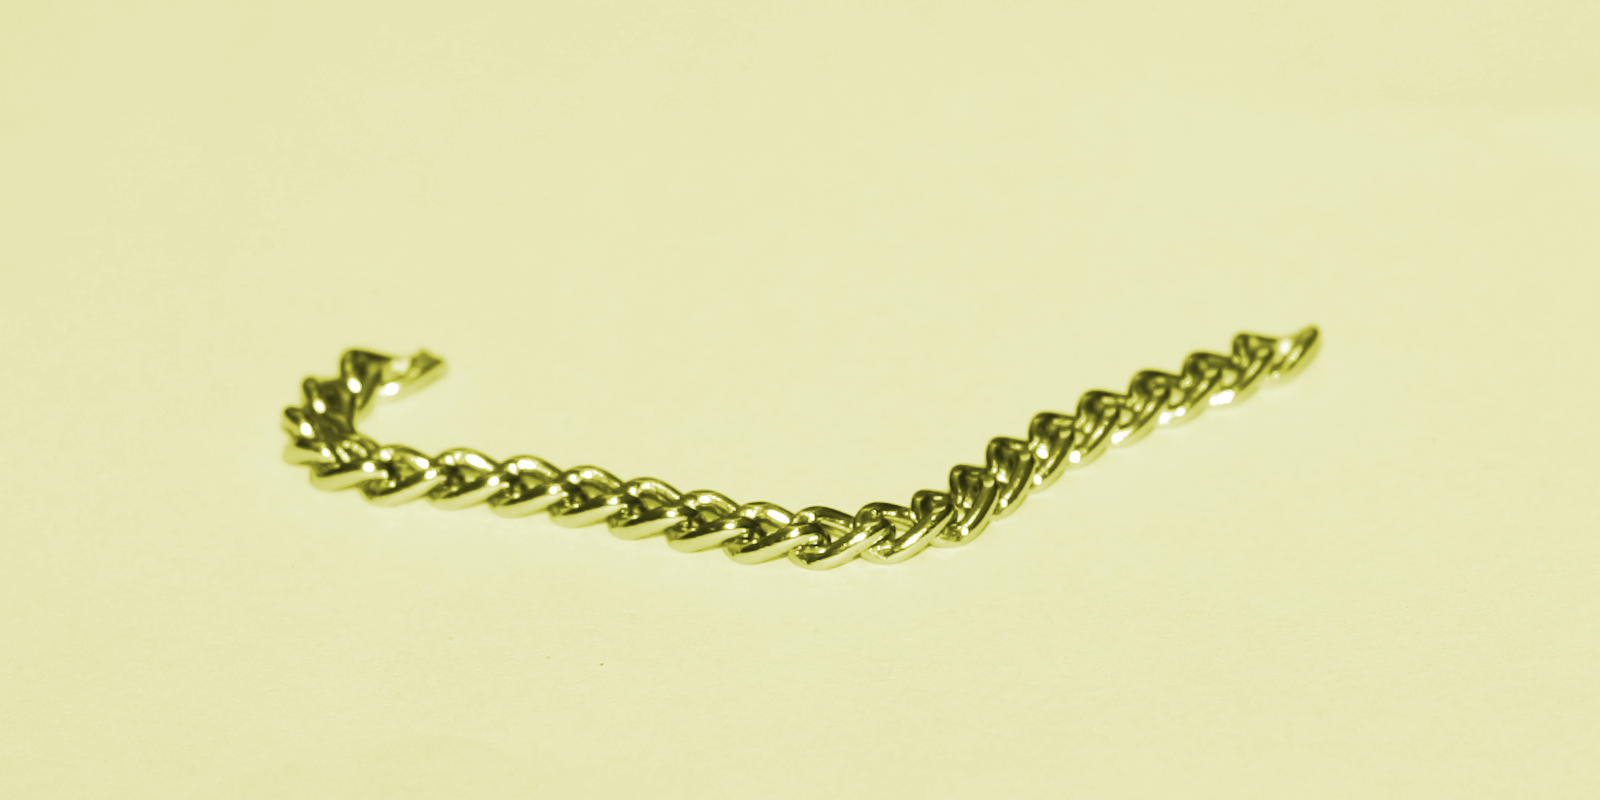
\includegraphics[width=\linewidth]{cadena23.png}
\end{center}
Se le ocurre una idea y decide ponerla en práctica. Habla con
la dueña del hotel y, entre ambos, concluyen que si le da un eslabón
de la cadena por día, cubre exactamente el valor diario que
paga por la habitación. Y de esa forma puede solventar su estadía
durante los veintitrés días. Sus padres le aseguran que el dinero
llegará en algún momento durante ese lapso.

Entonces, como sabe que recibirá el dinero, tiene la intención
de arruinar su cadena lo menos posible. Es decir, prefiere
hacer la menor cantidad de cortes posibles, de manera tal que
cada día la señora tenga en su poder tantos eslabones como días
le adeuda.

En realidad, perfecciona un poco su idea porque advierte que,
si la mujer le permite entregar un eslabón un día y al día siguiente
cuando deberá entregarle otro ella le devuelve el del día anterior
y acepta canjeárselo por una combinación de dos eslabones,
y así siguiendo, quizá pueda evitarse tener que cortar la cadena
todos los días.

Después de explicarle su idea (para dañar la cadena lo menos posible),
el acuerdo al que llega con la dueña es el siguiente: él puede darle
un eslabón por día, o puede darle un eslabón el día 1, el día 2 puede
pedirle ese eslabón y entregarle a cambio una pequeña cadena compuesta
por dos eslabones. El día 3 puede darle un eslabón solo (que junto con
los dos que ella tiene le servirían para pagar el tercer día) o puede
pedirle que le devuelva los dos que ella ya tiene y entregarle un
pequeño segmento (una ``minicadena'') con tres eslabones, y así
siguiendo, día por día. Lo único que debería importarle a la dueña es
tener en su poder cada día la cantidad de eslabones equivalente a la
cantidad de días que el estudiante estuvo en su hotel.


Ahora viene la pregunta: ¿cuál es el máximo número de cortes
que tiene que hacer el joven estudiante para arruinar su cadena lo
menos posible y honrar su acuerdo los veintitrés días?
\section*{Sudoku}
\begin{center}
  \begin{tikzpicture}[scale=.9]
  \begin{scope}
    \draw (0, 0) grid (9, 9);
    \draw[very thick, scale=3] (0, 0) grid (3, 3);

    \setcounter{row}{1}
    \setrow { }{2}{ }  {5}{ }{1}  { }{9}{ }
    \setrow {8}{ }{ }  {2}{ }{3}  { }{ }{6}
    \setrow { }{3}{ }  { }{6}{ }  { }{7}{ }

    \setrow { }{ }{1}  { }{ }{ }  {6}{ }{ }
    \setrow {5}{4}{ }  { }{ }{ }  { }{1}{9}
    \setrow { }{ }{2}  { }{ }{ }  {7}{ }{ }

    \setrow { }{9}{ }  { }{3}{ }  { }{8}{ }
    \setrow {2}{ }{ }  {8}{ }{4}  { }{ }{7}
    \setrow { }{1}{ }  {9}{ }{7}  { }{6}{ }

    \node[anchor=center] at (4.5, -0.5) {Sudoku 1};
  \end{scope}
\end{tikzpicture}\\
{\bf Las soluciones en el próximo número.}
\end{center}
\end{multicols}
\newpage

%%% Local Variables:
%%% mode: latex
%%% TeX-master: "jugando"
%%% End:



